\documentclass[tikz, border=4pt]{standalone}
\usepackage{tikz}
\usetikzlibrary{arrows.meta}
\begin{document}
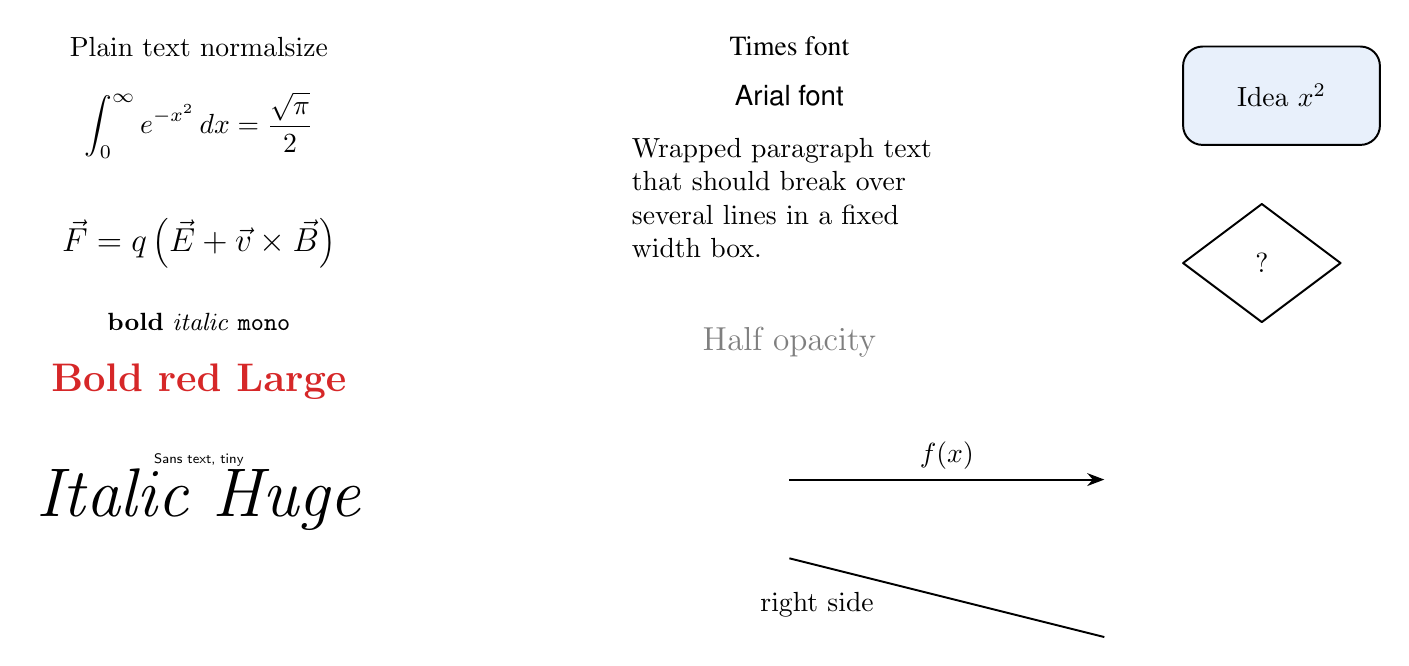
\begin{tikzpicture}[x=1cm, y=1cm]
  \definecolor{tdc1}{HTML}{D62728}
  \definecolor{tdc2}{HTML}{E8F0FB}

  \node at (0,0) {Plain text normalsize};
  \node at (0,-1) {$\displaystyle\int_0^\infty e^{-x^2}\,dx = \frac{\sqrt{\pi}}{2}$};
  \node[font=\large] at (0,-2.5) {$\vec F = q\left(\vec E + \vec v \times \vec B\right)$};
  \node[font=\small] at (0,-3.5) {\textbf{bold} \textit{italic} \texttt{mono}};
  \node[font=\Large\bfseries, text=tdc1] at (0,-4.25) {Bold red Large};
  \node[font=\tiny\sffamily] at (0,-5.25) {Sans text, tiny};
  \node[font=\Huge\itshape] at (0,-5.75) {Italic Huge};
  \node[font=\fontfamily{ptm}\selectfont] at (7.5,0) {Times font};
  \node[font=\fontfamily{phv}\selectfont] at (7.5,-0.62) {Arial font};
  \node[text width=4cm, align=left, inner sep=0pt, anchor=north] at (7.5,-1.16) {Wrapped paragraph text that should break over several lines in a fixed width box.};
  \node[font=\large, opacity=0.5] at (7.5,-3.75) {Half opacity};
  \draw[line width=0.71pt, -{Stealth}] (7.5,-5.5) -- node[auto, pos=0.5] {$f(x)$} (11.5,-5.5);
  \draw[line width=0.71pt] (7.5,-6.5) -- node[auto, swap, pos=0.3] {right side} (11.5,-7.5);
  \draw[line width=0.71pt, fill=tdc2, line join=round] (12.75,0) -- (14.75,0) -- (14.75,0) .. controls (14.89,0) and (15,-0.11) .. (15,-0.25) -- (15,-1) -- (15,-1) .. controls (15,-1.14) and (14.89,-1.25) .. (14.75,-1.25) -- (12.75,-1.25) -- (12.75,-1.25) .. controls (12.61,-1.25) and (12.5,-1.14) .. (12.5,-1) -- (12.5,-0.25) -- (12.5,-0.25) .. controls (12.5,-0.11) and (12.61,0) .. (12.75,0) -- cycle;
  \node[align=center] at (13.75,-0.62) {Idea $x^2$};
  \draw[line width=0.71pt, line join=round] (13.5,-2) -- (14.5,-2.75) -- (13.5,-3.5) -- (12.5,-2.75) -- cycle;
  \node[align=center] at (13.5,-2.75) {$?$};
\end{tikzpicture}
\end{document}
